\documentclass{article}
\usepackage[utf8]{inputenc}
\usepackage[english]{babel}

\usepackage{tikz}
\usetikzlibrary{graphs, positioning, arrows, matrix}

\usepackage{amssymb,latexsym,amsmath,amscd,amsthm, mathtools,stmaryrd, hyperref, enumitem, array, cleveref}

\theoremstyle{theorem}
\newtheorem{theorem}{Theorem}
\newtheorem{proposition}{Proposition}

\theoremstyle{definition}
\newtheorem{definition}{Definition}
\newtheorem{remark}{Remark}
\newtheorem{example}{Example}
\newtheorem{problem}{Problem}


%opening
\title{Supersingular Isogeny Diffie-Hellman}
\author{Valeriia Kulynych\\ Université de Toulon}

\begin{document}

\maketitle

\section{Supersingular Elliptic Curves}

\subsection{Various definitions}

Let $K$ be a field with algebraic closure $\bar{K}$.

\begin{definition}[Projective space]
	The \textit{projective space of dimension $n$}, denoted by $\mathbb{P}^n$ or $\mathbb{P}^n(\bar{K})$ is the set of all $(n+1)$-tuples
		\[ (x_0, \dots, x_n) \in \bar{K}^{n+1} \]
	such that $(x_0, dots, x_n) \neq (0, \dots, 0)$ taken modulo the equivalence relation 
		\[ (x_0, \dots, x_n) \sim (y_0, \dots, y_n) \]
	if and only in there exists $\lambda \in \bar{K}, \lambda \neq 0$ such that $x_i = \lambda y_i$ for all $i$ (Cf. \cite[I]{IsogenyCryptoDeFeo}).
\end{definition}


The equivalence class of a projective point $(x_0, \dots, x_n)$ is denoted by $[x_0, \dots, x_n]$. The set of $K$-rational points, denoted by $\mathbb{P}^n(K)$, is defined as 
	\[ \mathbb{P}^n(K) = \{ [x_0, \dots, x_n] \in \mathbb{P}^n | x_i \in K \ \text{for all} \ i \} \]

\begin{definition}[Elliptic curve] 
	An \textit{elliptic curve} is a pair $(E, O)$, where $E$ is a curve of genus 1 and $O \in E$. (We often just write $E$ for the elliptic curve, the point $O$ is being understood.) $E(K)$ is the subgroup of rational points over field $k$ on the curve $E$. The elliptic curve $E$ is defined over $K$, written $E/K$, if $E$ is defined over $K$ as a curve and $O \in E(K)$. (Cf. \cite[III, \S3]{Silverman}).
\end{definition}

Let $E$ be an elliptic curve given by a Weierstrass equation (see page \pageref{WE}). Remember that $E \subset \mathbb{P}^2$ consists of the points $P = (x, y)$ satisfying the Weierstrass equation together with the point $O = [0, 1, 0]$ at infinity. Let $L \subset \mathbb{P}^2$ be a line. Then since the equation has degree three, $L$ intersects $E$ at exactly 3 points, say $P, Q, R$. (Note if $L$ is tangent to $E$, then $P, Q, R$ may not be distinct. The fact that $L \cap E$ taken with multiplicities, consists of three points, is a special case of Bezout's theorem (Cf. \cite[I.7, Corollary 7.8]{Hartshorne}).

Define a composition law $\oplus$ on $E$ by the following rule.

\begin{definition}[Composition law]
	Let $P, Q \in E$, $L$ be the line connecting $P$ and $Q$ (tangent line to $E$ if $P = Q$), and $R$ be the third point of intersection of $L$ with $E$. Let $L'$ be the line connecting $R$ and $O$. Then $P \oplus Q$ is the point such that $L'$ intersects $E$ at $R, O \ \text{and} \ P \oplus Q$ (Cf. \cite[III, \S2]{Silverman}).
\end{definition}

Let $E$ be an elliptic curve defined over $K$. As $E$ with composition law $\oplus$ has an abelian group structure, then we can define subgroup of its rational points over the field $K$ and denote it $E(K)$. 

Now we assume that the characteristic of $K$ is $p > 0$.

	\begin{definition}[Supersingular elliptic curve] \label{ssedef1}
		For every $n$, we have a multiplication map 
		\[[n]: E \to E\]
		\[ P \mapsto \underbrace{P \oplus \cdots \oplus P}_{n \ \text{times}}. \]
		Its kernel is denoted by $E[n]$ and is called the $n$-torsion subgroup of $E$. Then one can show that for any $r \geq 1$:
		\[ E[p^r](\bar{K}) \simeq
			\begin{cases}
			{0} \\
			\mathbb{Z}/p^r\mathbb{Z}
		\end{cases} \]
		In the first case, $E$ is called \textit{supersingular}. Otherwise, it is called \textit{ordinary} (Cf. \cite[V, \S3, Theorem 3.1]{Silverman}).
	\end{definition}

For each integer $r \geq 1$ we consider the $p^r$-power Frobenius morphism (Cf. \cite[II, \S2]{Silverman}) given by  
	\[\phi_r: E \to E^{(p^r)}\]
	\[ [x_0, \dots, x_n] \mapsto [x_0^{p^r}, \dots, x_n^{p^r}] \]
Let $m = \mathrm{deg}\phi_r$. 
Then we consider the morphism
	\[\hat{\phi_r}: E^{(p^r)} \to E, \]
such that 
	\[ \hat{\phi_r} \circ \phi_r = [m], \]
where $[m]$ is $m$-multiplication map. Such $\hat{\phi_r}$ is called \textit{dual} of $p^r$-power Frobenius morphism (Cf. \cite[III, \S6, Theorem 6.1]{Silverman}). 

We remind that morphism $f: X \to Y$ is separable if $K(X)$ is a separable extension of $K(Y)$ (Cf. \cite[IV, 2]{Hartshorne}).

We remind the notion of separable extension. Let $F$ be a finite extension of $K$. We say that $F$ is separable over $K$ if $[F:K]_S = [F:K]$, where $[F:K]_S$ is a separable degree of $F$ over $K$. An element $\alpha$ algebraic over $K$ is said to be separable over $K$ if its minimal polynomial has no multiple roots.(Cf. \cite[V, \S4]{Lang}) Then one can show that $F$ is separable over $K$ if and only if each element of $F$ is sepable over $K$ (Cf. \cite[V, \S4, Theorem 4.3]{Lang}). Extensions which are not separable are called \textit{inseparable}.

A finite extension $K$ of field $k$ is \textit{purely inseparable} if for every $\alpha \in K$, $\alpha^{p^m} \in k$ for some $m \geq 0$ (Cf. \cite{PurelyInseparable}).
 
That brings us to another approach to define supersingular elliptic curve:
	\begin{definition}[Supersingular elliptic curve]
		An elliptic curve $E$ is supersingular if the map $\hat{\phi_r}$ is (purely) inseparable for one (all) $r \geq 1$ (Cf. \cite[V, \S3, Theorem 3.1]{Silverman}).
	\end{definition}

\begin{definition}[Weierstrass equation]\label{WE}
	An ellipric curve defined over $K$ is the locus in $\mathbb{P}^2$ of an equation
		\[ Y^2Z + a_1XYZ + a_3YZ^2 = X^3 + a_2X^2Z + a_4XZ^2 + a_6Z^3,  \]
	with $a_1,\dots, a_6 \in \bar{K}$. This equation is called a \textit{Weierstrass equation} (Cf. \cite[III, \S1]{Silverman}).
\end{definition} 

To ease notation, we will usually write the Weierstrass equation for our elliptic curve using non-homogeneous coordinates $x = X/Z$ and $y = Y/Z$, 
	\[ E: y^2 + a_1xy + a_3y = x^3 +a_2x^2 + a_4x +a_6, \]
always remembering that there is the extra point $O = [0, 1, 0]$ out at infinity. 

If $\mathrm{char}(\bar{K}) \neq 2$, then we can simplify the equation by completing the square. Replacing $y$ by $\frac{1}{2}(y - a_1x - a_3)$ gives an equation of the form
	\[E: y^2 = 4x^3 + b_2x^2 +2b_4x + b_6, \]
where
	\[b_2 = a_1^2 + 4a_2,\]
	\[b_4 = 2a_4 + a_1a_3,\]
	\[b_6 = a_3^2 + 4a_6.\]
We also define quantities
	\[b_8 = a_1^2a_6 + 4a_2a_6 - a_1a_3a_4 + a_2a_3^2 - a_4^2,\]
	\[c_4 = b_2^2 - 24b_4, \]
	\[c_6 = b_2^3 + 36b_2b_4 - 216b_6,\]
	\[\Delta = -b_2^2b_8 - 8b_4^3 - 27b_6^2 + 9b_2b_4b_6, \]
	\[j = c_4^2/\Delta.\]
%If further we have $\mathrm{char}(\bar{K}) \neq 2, 3$, then replacing $(x, y)$ by $(\frac{x - 3b_2}{36}, \frac{y}{216})$ eliminates the $x^2$ term, yielding the simpler equation
%	\[E: y^2 = x^3 - 27c_4x - 54c_6. \] 
	
The quantity $\Delta$ given above is called the \textit{discriminant} of the Weierstrass equation, $j$ is called the \textit{$j$-invariant} \label{j-invariant} of the elliptic curve $E$. Now we can given another one definition of a supersingular elliptic curve:
	\begin{definition}[Supersingular elliptic curve]
		If the map $[p]: E \to E$ is purely inseparable and $j(E) \in \mathbb{F}_{p^2}$ then the curve $E$ is called supersingular (Cf. \cite[V, \S3, Theorem 3.1]{Silverman}).
	\end{definition}


For the next definition of supersingular elliptic curve, we need to introduce the following notions. 

\begin{definition}[Order]
	Let $\mathcal{K}$ be a (not necessarily commutative) algebra (i.e. vector space equipped with a bilinear product), finitely generated over $\mathbb{Q}$. An \textit{order} $\mathcal{R}$ of $\mathcal{K}$ is a subring of $\mathcal{K}$ which is finitely generated as $\mathbb{Z}$-module (i.e. as an abelian group) and which satisfies $\mathcal{R} \otimes \mathbb{Q} = \mathcal{K}$, where $\otimes$ is the tensor product (Cf. \cite[III, \S9]{Silverman}).
\end{definition}

\begin{definition}[Quaternion algebra]
	A \textit{quaternion algebra} is an algebra of the form
	\[ \mathcal{K} = \mathbb{Q} +\mathbb{Q}\alpha + \mathbb{Q}\beta +\mathbb{Q}\alpha\beta \]
	with the multiplication rules
	\[ \alpha^2, \beta^2 \in \mathbb{Q}, \quad \alpha^2 < 0, \quad \beta^2 < 0, \quad \beta\alpha = - \alpha\beta. \] (Cf. \cite[III, \S9]{Silverman}).
\end{definition}

\begin{definition}[Supersingular elliptic curve]
	An elliptic curve $E$ is supersingular if the endomorphism		ring $\mathrm{End}_{\bar{K}}(E)$ is an order in a quaternion algebra (Cf. \cite[V, \S3, Theorem 3.1]{Silverman}).
\end{definition}

\begin{remark}
 	The endomorphism ring of an elliptic curve is either $\mathbb{Z}$ (if $p = 0$), an order in an imaginary quadratic number field (a number field of the form $\mathbb{Q}[\sqrt{-D}]$ for some $D > 0$), or an order in a quaternion algebra (Cf. \cite[III, \S, Corollary 9.4]{Silverman}).  
\end{remark}

Another way to define supersingular elliptic curve is based on a notion of a formal group.

Let $R$ be a ring of characteristic $p > 0$.
\begin{definition}[Formal group]
	 A \textit{(one-parameter commutative) formal group $\mathcal{F}$ defined over $R$} is a power series $F(X, Y) \in R\llbracket X, Y \rrbracket $ satisfying:
		\begin{enumerate}
			\item $F(X, Y) = X + Y + \ \text{(terms of degree} \ \geq 2)$.
			\item $F(X, F(Y, Z)) = F(F(X, Y), Z)$ (associativity).
			\item $F(X, Y) = F(Y, X)$ (commutativity).
			\item There is unique power series $i(T) \in R\llbracket T \rrbracket$ such that $F(T, i(T)) = 0$ (inverse).
			\item $F(X, 0) = 0$ and $F(0, Y) = Y$.
		\end{enumerate} \cite[IV, \S2]{Silverman}.
\end{definition}

We call $F(X,Y)$ the \textit{formal group law of $\mathcal{F}$}.
 
Returning now to formal power series, we look for the power series formally giving the addition law on E. Thus let $z_1, z_2$ be independent indeterminates, and let 
	\[w_i = w(z_i) = z_i^3(1 + A_1z_i + A_2z_i^2 + \cdots) \in \mathbb{Z}[a_1, \dots, a_6]\llbracket z_i \rrbracket,\]
where $A_i \in \mathbb{Z}[a_1, \dots, a_6]$, for $i = 1, 2$. In the $(z, w)$-plane, the line connecting $(z_1, w_1)$ to $(z_2, w_2)$ has slope
	\[ \lambda = \lambda(z_1, z_2) = \frac{w_2 - w_1}{z_2 - z_1} = \sum_{n = 3}^{\infty} A_n\frac{z_2^n -z_1^n}{z_2 - z_1} \in \mathbb{Z}[a_1, \dots, a_6]\llbracket z_1, z_2 \rrbracket. \]
Letting
	\[v = v(z_1, z_2) = w_1 - \lambda z_1 \in \mathbb{Z}[a_1, \dots, a_6]\llbracket z_1, z_2 \rrbracket, \]
the connecting line has equation $w = \lambda z +v$. Substituting this into the Weierstrass equation gives a cubic in $z$, two of whose roots are $z_1$ and $z_2$. Looking at the quadratic term, we see that the third $z_3$ can be expressed as a power series in $z_1$ and $z_2$:
	\[z_3 = z_3(z_1, z_2) =\]
	\[= -z_1 -z_2 + \frac{a_1\lambda + a_3\lambda^2 -a_2v - 2a_4\lambda v - 3a_6\lambda^2v}{1 + a_2\lambda + a_4\lambda^2 + a_6\lambda^3}\]
	\[\in \mathbb{Z}[a_1, \dots, a_6]\llbracket z_1, z_2 \rrbracket.\]
For the group law on $E$, the points $(z_1, w_1), (z_2, w_2), (z_3, w_3)$ add up to zero. Thus to add the first two, we need the formula for the inverse. In the $(x, y)$-plane, the inverse of $(x, y)$ is $(x, -y -a_1x - a_3)$. Hence the inverse of $(z, w)$ will have $z$-coordinate ($z = -x/y$)
	\[ i(z) = \frac{x(z)}{y(z) + a_1x(z) + a_3} = \frac{z^{-2} - a_1z^{-1} - \dots}{-z^{-3} + 2a_1z^{-2} + \dots } \]
This gives the formal additional law 
	\[F(z_1, z_2) = i(z_3(z_1, z_2)) = \]
	\[= z_1 + z_2 - a_1z_1z_2 - a_2(z_1^2z_2 + z_1z_2^2) - (2a_3z_1^3z_2 - (a_1a_2 - 3a_3)z_1^2z_2^2 + 2a_3z_1z_2^3) + \dots \]
	\[\in \mathbb{Z}[a_1, \dots, a_6] \llbracket z_1, z_2 \rrbracket. \]
Let $E$ be an elliptic curve given by a Weierstrass equation with coefficients in $R$. The \textit{formal group associated to $E$}, denoted $\hat{E}$, is given by the power series $F(z_1, z_2)$ described above.
 
\begin{definition}[Height of homomorphism; height of formal group]
	Let $\mathcal{F}, \mathcal{G}$ defined over $R$ be formal groups and $f: \mathcal{F} \to \mathcal{G}$ a homomorphism defined over $R$. The \textit{height of $f$}, denoted $ht(f)$, is the largest integer $h$ such that 
		\[f(T) = g(T^{p^h}) \]
	for some power series $g(T) \in R \llbracket T \rrbracket$. (If $f = 0$, then $ht(f) = \infty$.) The \textit{height of $\mathcal{F}$}, denoted $ht(\mathcal{F})$, is the height of the multiplication by $p$ map $[p]: \mathcal{F} \to \mathcal{F}$ \cite[IV, \S7]{Silverman}.
\end{definition}

	\begin{definition}[Supersingular elliptic curve]
		If the formal group $\hat{E}/K$ associated to $E$ has height 2, then $E$ is supersingular \cite[V, \S3, Theorem 3.1]{Silverman}. 
	\end{definition}

For the next approach to define supersingular curve we introduce an important invariant of elliptic curve $E$ defined over a perfect field $K$ of characteristic $p > 0$.

Let $F: E \to E$ be the Frobenius morphism. Then F induces a map:
	\[ F^{\ast}: H^1(E, \mathcal{O}_E) \to H^1(E, \mathcal{O}_E)  \]
on cohomology. This map is not linear, but it is \textit{$p$-linear}, namely $F^{\ast}(\lambda a) = \lambda^pF^{\ast}(a)$ for all $\lambda \in K, a \in H^1(E, O_E)$. Since $E$ is elliptic, $H^1(E, O_E)$ is a one-dimensional vector space. Thus, since $K$ is perfect, the map $F^{\ast}$ is either 0 or bijective.
For more information on cohomology see \cite[III]{Hartshorne}.
	\begin{definition}[Hasse invariant, Supersingular elliptic curve]
		If $F^{\ast} = 0$, we say that $E$ has \textit{Hasse invariant $0$} or that $E$ is \textit{supersingular}; otherwise we say that $E$ has \textit{Hasse invariant 1} \cite[IV, 4]{Hartshorne}.
	\end{definition}

The next theorem also could be used as a definition.
	\begin{theorem} 
		An elliptic curve $E/\mathbb{F}_q$ is supersingular if and only if $\mathrm{tr}\phi_E \cong 0 \mathrm{mod} p$, where $\phi_E$ is the Frobenius morphism (Cf. \cite[Lecture 14]{SutherlandEllipticCurves}).
	\end{theorem}
		\begin{proof}
			We first suppose that $E$ is supersingular and assume $q = p^n$ so that $\phi_E = \phi^n$. Then $\mathrm{ker}[p] = \mathrm{ker}\phi\hat{\phi}$ is trivial, and therefore $\mathrm{ker}\hat{\phi}$ is trivial. Thus $\hat{\phi}$ is inseparable, since it has degree $p > 1$. The isogeny (see \pageref{isogeny}) $\hat{\phi}^n = \hat{\phi^n} = \hat{\phi}_E$ is also inseparable,as is $\phi_E$, so $\mathrm{tr}\phi_E = \phi_E + \hat{\phi}_E$ is a sum of inseparable endomorphisms, hence inseparable (here we are viewing the integer $\mathrm{tr}\phi$ as an endomorphism). Therefore $\mathrm{deg}(\mathrm{tr}\phi_E) = (\mathrm{tr}\phi_E)^2$ is divisible by $p$, so $\mathrm{tr}\phi_E \cong 0 \mathrm{mod} p.$
			
			Conversely, if $\mathrm{tr}\phi_E \cong 0 \mathrm{mod} p$, then $p$ divides $\mathrm{deg}(\mathrm{tr}\phi_E) = (\mathrm{tr}\phi_E)^2$ and $\mathrm{tr}\phi_E$ is inseparable, as is $\hat{\phi}_E = \mathrm{tr}\phi_E - \phi_E$. This means that $\hat{\phi}^n$ and therefore $\hat{\phi}$ is inseparable. So $\mathrm{ker}\hat{\phi}$ is trivial, since it has prime degree $p$, and the same is true for $\phi$. Thus the kernel of $[p] = \hat{\phi}\phi$ is trivial and $E$ is supersingular.
		\end{proof}
		

When $q=p$ is a prime greater than 3 this is equivalent to having the trace of Frobenius morphism equal to zero; this does not hold for $p = 2 \ \text{or} \ 3$.

 \subsection{Examples}

In this section we are going to give some examples of supersingular curves.

Using definitions given in previous section may not always be a convenient way to identify a supersingular curves. But from those equivalent definitions we see thath up to isomorphism, there are only finitely many elliptic curves with Hasse invariant 0, since each has $j$-invariant in $\mathbb{F}_{p^2}$. For $p = 2$, once can easily check that the only one supersingular elliptic curve is 
	\[ E: y^2 + y = x^3. \]
For $p > 2$, the following theorem gives a simple criterion for determining whether an elliptic curve is supersingular.

\begin{theorem} \label{thm1}
	Let $K$ be finite field of characteristic $p > 2$.
		\begin{enumerate}[label = (\alph*)]
			\item Let $E/K$ be an elliptic curve with Weierstrass equation 
					\[ E: y^2 = f(x) \]
				where $f(x) \in K[x]$ is a cubic polynomial with distinct roots (in $\bar{K}$). Then $E$ is supersingular if and only if the coefficient of $x^{p - 1}$ in $f(x)^{(p - 1)/2}$ is zero.
			
			\item  Let $m = (p - 1)/2$, and define a polynomial
					\[H_p(t) = \sum_{i = 0}^{m} \binom{m}{i}^2t^i. \]
				Let $\lambda \in \bar{K}$, $\lambda \neq 0, 1$. Then the elliptic curve
					\[E: y^2 = x(x - 1)(x - \lambda)  \]
				is supersingular if and only if $H_p(\lambda) = 0$.
			
			\item The polynomial $H_p(t)$ has distinct roots in $\bar{K}$. Up to isomorphism, there are exactly
					\[ [\frac{p}{12}] + \varepsilon_p \]
				supersingular elliptic curves in characteristic $p$, where $\varepsilon_p = 1$, and for $p \geq 5$,
					\[\varepsilon_p = 0, 1, 1, 2 \quad \textrm{if} \quad p \cong 1, 5, 7, 11 (\mathrm{mod}12). \]
			(Cf. \cite[V, \S4, Theorem 4.1]{Silverman})
		\end{enumerate}
\end{theorem}

\begin{example}
	For which primes $p \geq 5$ is the elliptic curve
		\[E:  y^2 = x^3 + 1\]
	supersingular?
	
	Notice this curve has $j(E) = 0$. From the criterion of \cref{thm1}(a), we must compute the coefficient of $x^{p-1}$ in $(x^3 + 1)^{(p-1)/2}$. If $p \cong 2 \mathrm{mod} 3$, then there is no $x^{p-1}$ term, so $E$ is supersingular; while if $p \cong 1 \mathrm{mod} 3$, then the coefficients is $\binom{(p-1)/2}{(p-1)/3}$, which is non-zero modulo $p$, so in this case $E$ is ordinary.
\end{example}

\begin{example}
	Similary we compute for which primes $p \geq 3$ the $j = 1728$ elliptic curve
		\[E: y^2 = x^3 + x \]
	is supersingular.
	
	This is determined by the coefficient of $x^{(p-1)/2}$ in $(x^2 + 1)^{(p-1)/2}$, which equals $0$ if $p \cong 3 \mathrm{mod} 4$ and $\binom{(p-1)/2}{(p-1)/4}$ if $p \cong 1 \mathrm{mod} 4$. Hence $E$ is supersingular if $p \cong 3 \mathrm{mod} 4$ and ordinary if $p \cong 1 \mathrm{mod} 4$.
\end{example}

\begin{example}
	Let $E$ be given by the equation 
		\[E: y^2 + y = x^3 -x^2 -10x - 20,\]
	so $j(E) = -\frac{2^{12}31^3}{11^5}$. Then by using the criterion of \cref{thm1} (a) directly one finds that the only primes $p < 100$ for which $E$ is supersingular in characteristic $p$ are $p = 19$ and $p = 29$. (D. H. Lehmer has calculated that there are exactly $27$ primes $p < 31500$ for which this $E$ is supersingular.) 
\end{example}


\section{Isogeny Graphs}

We start this section with a notion of isogeny.
	\begin{definition} \label{isogeny}
		Let $E_1$ and $E_2$ be elliptic curves defined over a finite field $\mathbb{F}_q$ of characteristic $p$. An \textit{isogeny} $\phi: E_1 \to E_2$ defined over $\mathbb{F}_q$ is a non-constant morphism that maps the identity into the identity (and this a is group homomorphism) (Cf. \cite[2.1]{HardEasyProbs}).
	\end{definition}
Two elliptic curves $E_1$ and $E_2$ defined over $\mathbb{F}_q$ are said to be \textit{isogenous} over $\mathbb{F}_q$ if there exists an isgony $\phi: E_1 \to E_2$ defined over $\mathbb{F}_q$.

\begin{theorem}[Sato-Tate]
	Two elliptic curves $E_1$ and $E_2$ are isogenous over $\mathbb{F}_q$ if and only if $\#E_1(\mathbb{F}_q) = \#E_2(\mathbb{F}_q)$ (Cf. \cite[Theorem 13]{IsogenyCryptoDeFeo}). 
\end{theorem}  

The degree of an isogeny $\phi$ is the degree of $\phi$ as a morphism. An isogeny of degree $\ell$ is called $\ell$-isogeny. 

Curves in the same isogeny class are either all supersingular or all ordinary.

%For prime $\ell \not| p$, we have $E[\ell] \simeq \mathbb{Z}/\ell\mathbb{Z} \oplus \mathbb{Z}/\ell\mathbb{Z}$ \cite[2]{TowardsQuantumRes}.

%Supersingular curves are all defined over $\mathbb{F}_{p^2}$, and for every prime $\ell \not| p$, there exist $\ell + 1$ isogenies (counting multiplicities) of degree $\ell$ originating from any given such supersingular curve. An isogeny can be identified with its kernel. Given a subgroup $G$ of $E$, we can use Velu's formulas \cite[Proposition 39]{IsogenyCryptoDeFeo} to compute an isogeny $\phi: E_1 \to E_2$ with kernel $G$ and such that $E_2 \simeq E_1/G$. 

For each isogeny $\phi: E_1 \to E_2$, there is a unique isogeny $\hat{\phi}: E_2 \to E_1$ which is called the \textit{dual isogeny} of $\phi$, satisfying $\phi\hat{\phi} = \hat{\phi}\phi = [\mathrm{deg}\phi]$. 

If we have two isogenies $\phi: E_1 \to E_2$ and $\phi': E_2 \to E_1$ such that $\phi\phi'$ and $\phi'\phi$ are the identity in their respective curves, we say that $\phi$, $\phi'$ are \textit{isomorphisms}, and that $E$, $E'$ are \textit{isomorphic}. Isomorphism classes of elliptic curves over $\mathbb{F}_q$ can be labeled with their $j$-invariants (see page \pageref{j-invariant}). In this paper we write $j(E)$ for the $j$-invariant of $E$. By convention given a $j$-invariant $j \neq 0, 1728$, we write $E(j)$ for the curve defined by the equation 
	\[y^2 = x^3 + \frac{3j}{1728 - j}x + \frac{2j}{1728 - j}. \]
We also write $E(0)$ and $E(1728)$ for the curves with equations
	\[y^2 = x^3 + 1 \quad \text{and} \quad y^2 = x^3 +x \]
respectively.

	\begin{definition}[Isogeny graph]
		Let $E$ be an elliptic curve over a field $K$ of characteristic $p$. Let $S \subseteq \mathbb{N}$ be a finite set of primes. Define
			\[X_{E, K, S} \]
		to be the graph with vertex set being the $K$-isogeny class of $E$. Vertices are typically labelled by $j(E)$, though we also speak of "the vertex $E$". There is an edge $(j(E_1), j(E_2))$ labelled by $\ell$ for ezch equivalence class of $\ell$-isogenies from $E_1$ to $E_2$ defined over $K$ for some $\ell \in S$. We usually treat this as an undirected graph, since for every $\ell$-isogeny $\phi: E_1 \to E_2$ there is a dual isogeny $\hat{\phi}: E_2 \to E_1$ of degree $\ell$ (Cf. \cite[25.2]{Galbraith-PKC}). 
	\end{definition}

\subsection{Supersingular isogeny graph}

For the supersingular isogey graph we work over $\bar{\mathbb{F}}_p$. The graph is finite. Indeed, \cref{thm1} (c) implies $\frac{p}{12} - 1 < \#X_{E, \bar{\mathbb{F}}_p, S} < \frac{p}{12} + 2$. Note that it suffices to consider elliptic curves defined over $\mathbb{F}_{p^2}$ (although the isogenies between them are over $\bar{\mathbb{F}}_p$ in genereal).

In contrast to the ordinary case , the supersingular graph is always connected using isogenies of any fixed degree (Cf. \cite[2.4]{Mestre}).

\begin{theorem}
	Let $p$ be a prime and let $E$ and $\tilde{E}$ be supersingular elliptic curves over $\bar{\mathbb{F}}_p$. Let $\ell$ be a prime different from $p$. Then there is an isogeny from $E$ to $\tilde{E}$ over $\bar{\mathbb{F}}_p$ whose degree is a power of $\ell$ (Cf. \cite[2.4]{Mestre}).
\end{theorem}

Hence, one can choose any prime $\ell$ and consider the $\ell$-isogeny graphh $X_{e,\bar{\mathbb{F}}_p, {\ell}}$ on supersingular curves over $\bar{\mathbb{F}}_p$. It follows that the graph is $(\ell + 1)$-regular and connected.

Now we will give some examples of supersingular isogeny graphs (cf. \cref{SIG83.figure}, \cref{SIG103.figure}, \cref{SIG101.figure})

\begin{figure}[h]
\begin{center}
	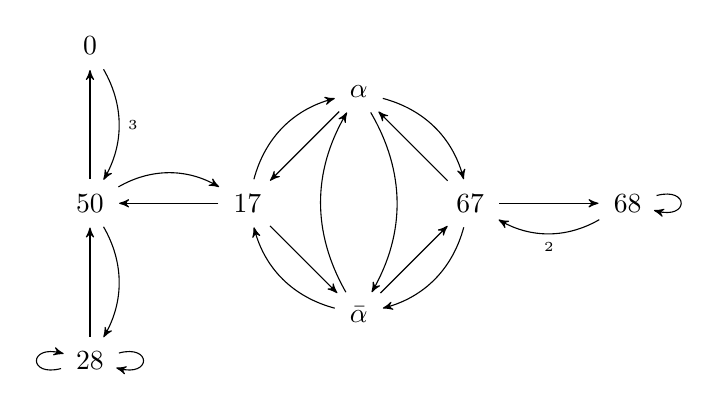
\begin{tikzpicture}[->, shorten >=2pt, shorten <=2pt, >=stealth', node distance = 2cm]

		\node (1) {$17$};
		\node (2) [above right of=1] {$\alpha$};
		\node (3) [below right of=1] {$\bar{\alpha}$};
		\node (4) [below right of=2] {$67$};
		\node (5) [right of=4] {$68$};
		\node (6) [left of=1] {$50$};
		\node (7) [below of=6] {$28$};
		\node (8) [above of=6] {$0$};

			\path
				(1) edge [bend left] (2)
				(1) edge (3)
				(1) edge (6)
				
				(2) edge (1)
				(2) edge [bend left] (3)
				(2) edge [bend left] (4)
				
				(3) edge [bend left] (1)
				(3) edge [bend left] (2)
				(3) edge (4)
				
				(4) edge (2)
				(4) edge [bend left] (3)
				(4) edge (5)
				
				(5) edge [bend left] node[below]{\tiny{$2$}} (4)
				(5) edge [loop right] (5)
				
				(6) edge [bend left] (1)
				(6) edge [bend left] (7)
				(6) edge (8)
				
				(7) edge (6)
				(7) edge [loop left] (7)
				(7) edge [loop right] (7)
				
				(8) edge [bend left] node[right]{\tiny{$3$}} (6);
  
\end{tikzpicture}
\end{center}
\caption{Supersingular Isogeny Graph $X_{\bar{\mathbb{F}}_{83}, 2}$}\label{SIG83.figure}
\end{figure}

\begin{figure}[h]
	\begin{center}
		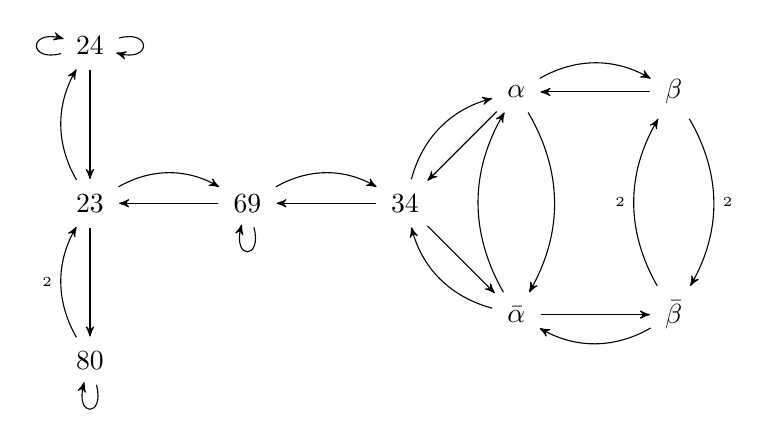
\begin{tikzpicture}[->, shorten >=2pt, shorten <=2pt, >=stealth', node distance = 2cm]
				
				\node (1) {$69$};
				\node (2) [right of=1] {$34$};
				\node (3) [above right of=2] {$\alpha$};
				\node (4) [below right of=2] {$\bar{\alpha}$};
				\node (5) [right of=3] {$\beta$};
				\node (6) [right of=4] {$\bar{\beta}$};
				\node (7) [left of=1] {$23$};
				\node (8) [above of=7] {$24$};
				\node (9) [below of=7] {$80$};
				
					\path
						(1) edge [loop below] (1)
						(1) edge [bend left] (2)
						(1) edge (7)
						
						(2) edge (1)
						(2) edge [bend left] (3)
						(2) edge (4)
						
						(3) edge (2)
						(3) edge [bend left] (4)
						(3) edge [bend left] (5)
						
						(4) edge [bend left] (2)
						(4) edge [bend left] (3)
						(4) edge (6)
						
						(5) edge (3)
						(5) edge [bend left] node[right] {\tiny{$2$}} (6)
						
						(6) edge [bend left] (4)
						(6) edge [bend left] node[left] {\tiny{$2$}} (5)
						
						(7) edge [bend left] (1)
						(7) edge [bend left] (8)
						(7) edge (9)
						
						(8) edge (7)
						(8) edge [loop left] (8)
						(8) edge [loop right] (8)
						
						(9) edge [bend left] node[left] {\tiny{$2$}} (7)
						(9) edge [loop below] (9);
				
		\end{tikzpicture}
	\end{center}
\caption{Supersingular Isogeny Graph $X_{\bar{\mathbb{F}}_103, 2}$}\label{SIG103.figure}
\end{figure}

\begin{figure}[h]
	\begin{center}
		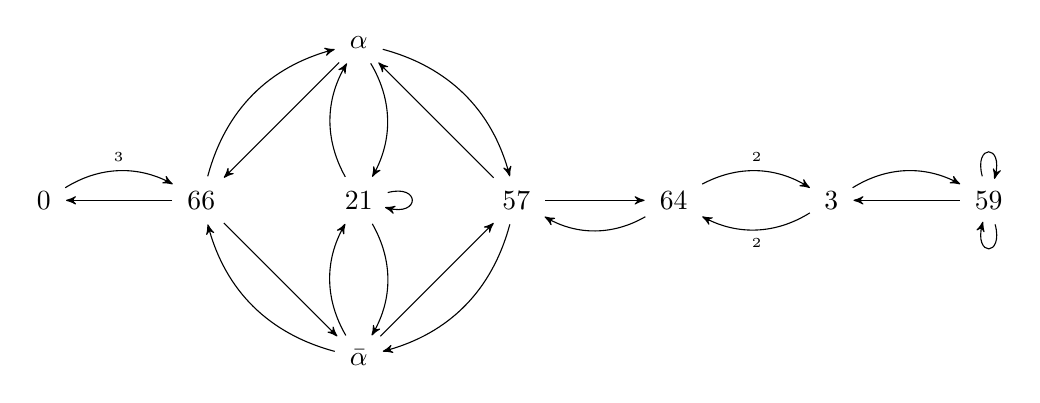
\begin{tikzpicture}[->, shorten >=2pt, shorten <=2pt, >=stealth', node distance = 2cm]
		
			\node (1) {$57$};
			\node (2) [left of=1] {$21$};
			\node (3) [above of=2] {$\alpha$};
			\node (4) [below of=2] {$\bar{\alpha}$};
			\node (5) [left of=2] {$66$};
			\node (6) [left of=5] {$0$};
			\node (7) [right of=1] {$64$};
			\node (8) [right of=7] {$3$};
			\node (9) [right of=8] {$59$};
			
				\path
					(1) edge (3)
					(1) edge [bend left] (4)
					(1) edge (7)
					
					(2) edge [loop right] (2)
					(2) edge [bend left] (3)
					(2) edge [bend left] (4)
					
					(3) edge [bend left] (1)
					(3) edge [bend left] (2)
					(3) edge (5)
					
					(4) edge (1)
					(4) edge [bend left] (2)
					(4) edge [bend left] (5)
					
					(5) edge [bend left] (3)
					(5) edge (4)
					(5) edge (6)
					
					(6) edge [bend left] node[above] {\tiny{$3$}} (5)
					
					(7) edge [bend left] (1)
					(7) edge [bend left] node[above] {\tiny{$2$}} (8)
					
					(8) edge [bend left] node[below] {\tiny{$2$}} (7)
					(8) edge [bend left] (9)
					
					(9) edge (8)
					(9) edge [loop above] (9)
					(9) edge [loop below] (9);
					
		
		\end{tikzpicture}
	\end{center}
\caption{Supersingular Isogeny Graph $X_{\bar{\mathbb{F}}_{101}, 2}$}\label{SIG101.figure}
\end{figure}

\section{Application: Diffie-Hellman key exchange}

Elliptic curves are widely used in modern cryptography. One of the most famous applications of the elliptic curves in cryptography is \textit{Diffie-Hellman key exchange}, a cryptographic protocol by which two parties communicating over a public channel can agree on a common secret string unknown to any other party listening on the same channel.

\subsection{Classic Diffie-Hellman}

We will first consider the original protocol, which was invented in the 1970s by Whitfield Diffie and Martin Hellman (cf. \cite{DiffieHellman}), and constitutes the first practical example of public key cryptography. The two communicating parties are customarily called \textit{Alice} and \textit{Bob}, and the listening third party is a character called \textit{Eve}. 

Firstly, Alice and bob agree on a set of public parameters:
	\begin{itemize}
		\item A large enough prime number $p$, such that $p - 1$ has a large enough prime faactor;
		
		\item A multiplicative generator $g \in \mathbb{Z}/p\mathbb{Z}$.
		
	\end{itemize}
Then, Alice and Bob perform the following steps:
	
	\begin{enumerate}
		\item Each chooses a \textit{secret} integer in the interval $]0, p - 1[$: called $a$ \textit{Alice's secret} and $b$ \textit{Bob's secret}.
		
		\item They respectively compute $A = g^a$ and $B = g^b$.
		
		\item They exchange $A$ and $B$ over the public channel.
		
		\item They respectively compute the \textit{shared secret} $B^a = A^b = g^{ab}$.
	\end{enumerate}

The protocol can be generalized by replacing the multiplicative group $(\mathbb{Z}/p\mathbb{Z})^{\ast}$ with anny other cyclic group $G = \langle g \rangle$. So Eve is given the knowledge of the group $G$, its generator $g$ and public data $A, B \in G$. Her goal is to recover the shared secret $g^{ab}$, which is mathematically possible, but not always easy to compute.

\begin{definition}[Discrete logarithm]
	Let $G$ be a cycluc group generated by an element $g$. For any element $A \in G$, we define the \textit{dicrete logarithm of $A$ in base $g$}, denoted $\log_g(A)$, as the unique integer in the interval $[0, \#G[$ such that
		\[ g^{\log_g(A)} = A. \] 
\end{definition}

It is obvious that if Eve can compute discrete logarithms in $G$ efficiently, the she can also compute the shared secret. Thus, the strenth of the Diffie-Hellman key exchange protocol is entirely dependent on the hardness of the dicrete logarithm promblem in the group $G$.

There exists some algorithms to compute discrete logarithms in a generic group $G$ that require $O(\sqrt{q})$ computational steps (see \cite{Joux}), where $q$ is the largest prime divisor of $\#G$. We also know that these algorithms are optimal for abstract cyclic groups. Therefore, the group $G$ is usually chosen that way that the largest prime divisor $Q$ has size at least $\log_2q \simeq 256$. But there also exist algorithms of complexity better than $O(\sqrt{\#G})$ for the case $G = (\mathbb{Z}/p\mathbb{Z})^{\ast}$ (see \cite{Joux}), thus requiring parameters of larger size to guarantee cryptographic strength.

\subsection{Elliptic Curve Diffie-Hellman}

However, no algorithms that solve discrete algorithm problem then generic ones are known for the case when $G$ is a subgroup of $E(K)$, where $E$ is an elliptic curve defined over a finite field $K$. For this reason, in the 1980s Miller (\cite{Miller}) and Koblitz (\cite{Koblitz}) suggested to replace $(\mathbb{Z}/p\mathbb{Z})^{\ast}$ in the Diffie-Hellman protocol by the group of rational point of an elliptic curve over a finite field. In this case public parameters of Elliptic Curves Diffie-Hellman (ECDH) protocol are:

	\begin{itemize}
		\item Finite field $\mathbb{F}_p$, with $\log_2p \simeq 256$;
		
		\item Elliptic curve $E$ over the finite field $\mathbb{F}_p$, such that $\#E(\mathbb{F}_p)$ is prime;
		
		\item A generator $P$ of $E(\mathbb{F}_p)$.
	\end{itemize} 

And then Alice and Bob take the following steps:

	\begin{enumerate}
		\item Each chooses a secret from $]0, \#E(\mathbb{F}_p)[$, where we denote Alice's secret as $a$, and Bob's as $b$.
		
		\item They compute public data $A = [a]P$ and $B = [b]P$.
		
		\item Alice and Bob exchange public data.
		
		\item Finally, they compute shared secret $S = [a]B = [b]A$.
	\end{enumerate}

It is already known that it is possible to reduce discrete logarithm problem on supersingular elliptic curves to the discrete logarithm problem in finite field (Cf. \cite{MOV}). Hence it is possible to reduce the problem to one which is known to have sub-exponential complexity. That is why one should avoid using supersingular curves in ECDH.

\subsection{Supersingular Isogeny Diffie-Hellman}

%This paper concerns on using isogenies between \textit{supersingular} elliptic curves instead of ordinary elliptic curves. The main technical difficulty is that, in the supersingular case, the endomorphism ring is noncommutative, whereas Diffie-Hellman type require commutativity.

Before moving to the Supersingular Isogeny Diffie-Hellman protocol description, we recall some concepts of graph theory.

We will restrict to undirected graphs. The \textit{diameter} of a connected graph is the largest of all distances between its vertices. A \textit{path} in undirected graph $(E, V)$ between two vertices $v, v'$ is a sequence of vertices $v \to v_1 \to \cdots \to v'$such that each vertex is connected to the next  by an edge. The \textit{adjacency matrix} of a graph $G$ with vertex set $V = {v_1, \dots, v_n}$ and edge set $E$, is $n \times n$ matrix where the $(i, j)$-th entry is 1 if there is an edge between $v_i$ and $v_j$, and 0 otherwise. Since we have restricted to undirected graphs, the adjacency matrix is symmetric, thus it has $n$ real eigenvalues
	\[ \lambda_1 \geq \dots \geq \lambda_n. \]
It is convenient to identify functions on $V$ with vectors in $\mathbb{R}^n$, and therefore consider the adjacency matrix as a self-adjoint operator in $L^2(V)$. Then we can bound the eigenvalues of $G$.

\begin{proposition}
	if $G$ is a $k$-regular graph, then its largest and smallest eigenvalues $\lambda_1$ and $\lambda_n$ satisfy
		\[ k = \lambda_1 \geq \lambda_n \geq -k. \]
		(Cf. \cite{Tao})
\end{proposition}

\begin{definition}[Expander graph]
	Let $\varepsilon > 0$ and $k \geq 1$. A $k$-regular graph is called a \textit{(one-sided) $\varepsilon$-expander} if
		\[ \lambda_2 \leq (1 - \varepsilon)k \]
	and a \textit{two-sided $\varepsilon$-expander} if it also satisfies
		\[ \lambda_n \geq -(1 - \varepsilon)k. \]
\end{definition}

A sequence $G_i = (V_i, E_i)$ of $k$-regular graphs with $\#V_i \to \infty$ is said to be a one-sided (respectively two-sided) \textit{expander family} if there is an $\varepsilon > 0$ such that $G_i$ is a one-sided (respectively two-sided) $\varepsilon$-expander for all sufficiently large $i$.

Expander families have a lot of applications in theoretical computer science due to their pseudo-randomness propreties: they are useful for pseudo-random number generators contructions, error-correcting codes, probabilistic checkable proofs and cryptographic primitives. We can describe them as having shoert diameter and rapidly mixing walks.

\begin{proposition}
	Let $G$ be a $k$-regular one sided $\varepsilon$-expander. For any vertex $v$ and eny radius $r > 0$, let $B(v, r)$ be the ball of vertices at distance at most $r$ from $v$. Then, there is a constant $c > 0$, depending  only on $k$ and $\varepsilon$, such that
		\[ \#B(v, r) \geq\min((1 + c)^r, \#V). \]
\end{proposition}

This shows that the diameter of an expander graph is bounded by $O(\log n)$, where the constant depends only on $k$ and $\varepsilon$. A \textit{random walk} of length $i$ is a path $v_1 \to \cdots v_i$, defined by the random process that selects $v_i$ uniformly at random among the neighbors of $v_{i-1}$. The next proposition says that, in an expander graph, random walks of length close to its diameter terminate on any vertex with probability close to uniform.

\begin{proposition}
	Let $G = (V, E)$ be a $k$-regular two-sided $\varepsilon$-expander. Let $F \subset V$ be any subset of the vertices of $G$, and let $v$ be any vertex in $V$. Then a random walk of length at least
		\[ \frac{\log\#F^{1/2}/2\#V}{\log(1 - \varepsilon)} \]
	starting from $v$ will land in $F$ with probability at least $\#F/2\#V$.
\end{proposition}

Now we come to one of the most powerful applications of isogeny graphs. There exist at least two key exchange protocols somewhat similar to the Diffie-Hellman protocol. Both of them are significantly less efficient than ECDH, but nevertheless they are relecant because of their conjectured \textit{quantum security}. %ADD THERE SOMETHING ABOUT QUANTUM-SECURITY 
The fisrt one was proposed by Rostovtsev and Stolbunov in  \cite{RostovstsevStolbunov}, but we will discuss only the second one, which first was introduced by Jao and De Feo in \cite{TowardsQuantumRes}.

We said that one should avoid supersingular ellipric curves in ECDH. But when we come to isogeny graphs, compared to the ordinary case, graphs of supersingular isogenies have two attractive features for constructing key exchange protocols. 
	\begin{itemize}
		\item One isogeny degree is sufficient to obtain an expander graph. BY choosing one small prime degree, we have the opportunity to construct more efficient protocols.
		
		\item  There is no action of an abelian group on them, so it seems harder to use quantum computers to speed up the supersingular isogeny path problem.
	\end{itemize}

It turns out that there is an algebraic structure acting on supersingular graphs. We have seen that, if $E$ is a supersingular curve defined over $\mathbb{F}_p$ or $\mathbb{F}_{p^2}$, then its endomorphism ring $End(E)$ is isomorphic to an order in the quaternion algebra $\mathbb{Q}_{p,\infty}$, ramified at $p$ and at infinity. Moreover, supersingular curves are in correspondence with the maximal orders of $\mathbb{Q}_{p, \infty}$and their left ideals act on the graph like isogenies.

The key idea of the Supersingular Isogeny Diffie-Hellman protocol (SIDH) is to let Alice and Bob take random walks in two distinct isogeny graphs on the same vertex set. In practice we choose a large enough prime $p$, and two small primes $\ell_A$ and $\ell_B$. The vertex set consists of the supersingular $j$-invariants defined over $\mathbb{F}_{p^2}$. Alice's graph is the graphs made of $\ell_A$-isogenies, and Bob's is made of $\ell_B$-isogenies. A very simple example of such graphs is shown on \cref{SIG97-2-3:figure}, where $p = 97, \ell_A = 2$ and $\ell_B = 3$.

\begin{figure}[h]
	\centering
	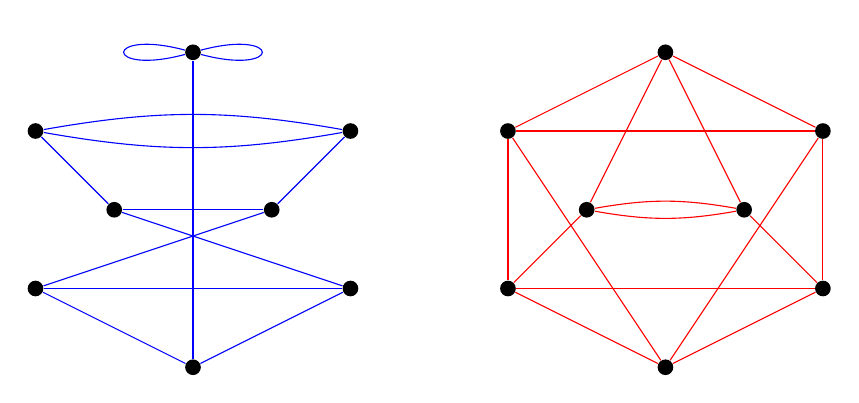
\begin{tikzpicture}
	\def\graph{
		\begin{scope}[every node/.style={fill,black,circle,inner sep=2pt}]
		\node at (0,0)  (1){};
		\node at (0,4) (20){};
		\node at (2,1)  (16z){};
		\node at (-2,1)  (81z){};
		\node at (-1,2) (77z){};
		\node at (1,2)  (20z){};
		\node at (-2,3)  (85z){};
		\node at (2,3)  (12z){};
		\end{scope}
	}
	
	\graph
	\begin{scope}[blue,every loop/.style={looseness=50}]
	\path (1) edge (20) edge (16z) edge (81z);
	\path (20) edge[loop left] (20) edge[loop right] (20);
	\path (16z) edge (81z) edge (77z);
	\path (81z) edge (20z);
	\path (77z) edge (20z) edge (85z);
	\path (20z) edge (12z);
	\path (12z) edge[bend right=10] (85z) edge[bend left=10] (85z);
	\end{scope}
	
	\begin{scope}[xshift=6cm]
	\graph
	\begin{scope}[red]
	\path (1) edge (85z) edge (81z) edge (12z) edge (16z);
	\path (20) edge (85z) edge (77z) edge (20z) edge (12z);
	\path (81z) edge (85z) edge (77z) edge (16z);
	\path (85z) edge (12z);
	\path (12z) edge (16z);
	\path (16z) edge (20z);
	\path (20z) edge[bend right=10] (77z) edge[bend left=10] (77z);
	\end{scope}
	\end{scope}
	\end{tikzpicture}
	\caption{Supersingular isogeny graphs of degree 2 (left, blue) and 3
		(right, red) on $\mathbb{F}_{97^2}$.}
	\label{SIG97-2-3:figure}
\end{figure}

But this information is not sufficient to define a key exchange protocol, because there is no canonical way of labeling the edges of these graphs. For this purpose we introduce a construction that uses the group structure of elliptic curves. Recall that a separable isogeny $\phi$ is uniquelly defined by its kernel and that in this case $\deg\phi = \ker\phi$. A walk of length $\varepsilon_A$ in the $\ell_A$-isogeny graph corresponds to a kernel of a size $\ell_A^{\varepsilon_A}$, and this kernel is cyclic if and only if the walk does not backtrack.

For this reason, if Alice chooses a secret walk of length $\varepsilon_A$ it is equivalent to choosing a secret cyclic subgroup $\langle A \rangle \subset E[\ell_A^{\varepsilon_A}]$. Bob respectively chooses his own secret $\langle B \rangle \subset E[\ell_B^{\varepsilon_B}]$, then there is a well defined subgroup $\langle A \rangle + \langle B \rangle = \langle A, B \rangle$, defining an isogeny to $E/\langle A, B \rangle$. Since we choose $\ell_A \neq \ell_B$, the group $\langle A, B \rangle$ is cyclic of order $\ell_A^{\varepsilon_A} \ell_B^{\varepsilon_B}$. This is illustrated in \cref{SIDH-diagram:figure}.

\begin{figure}
	\centering
	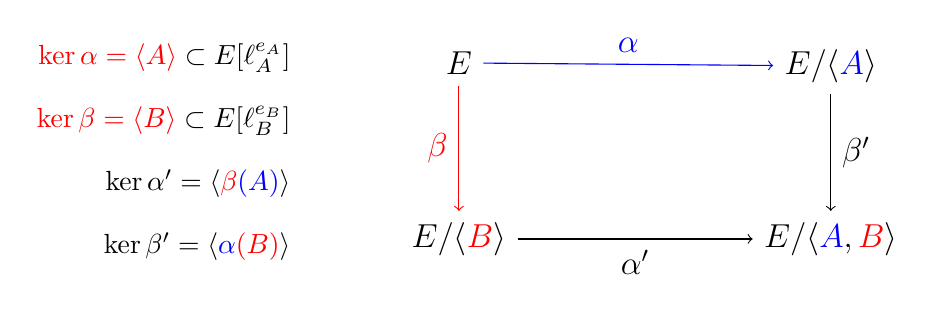
\begin{tikzpicture}
	
		\begin{scope}
			\draw (0,1.2) node[anchor=east] {$\textcolor{red}{\ker \alpha=\langle A\rangle} \subset E[\ell_A^{e_A}]$};
			
			\draw (0,0.4) node[anchor=east] {$\textcolor{red}{\ker \beta=\langle B\rangle} \subset E[\ell_B^{e_B}]$};
			
			\draw (0,-0.4) node[anchor=east] {$\ker \alpha' = \langle\textcolor{red}{\beta}\textcolor{blue}{(A)}\rangle$};
			
			\draw (0,-1.2) node[anchor=east] {$\ker \beta' = \langle\textcolor{blue}{\alpha}\textcolor{red}{(B)}\rangle$};
		\end{scope}
		
		\begin{scope}[xshift=4.5cm]
			\large
			\node[matrix of nodes, ampersand replacement=\&, column sep=3cm, row sep=1.5cm] (diagram) {
				|(E)| $E$ \& |(Es)| $E/\langle\textcolor{blue}{A}\rangle$ \\
				|(Ep)| {$E/\langle\textcolor{red}{B}\rangle$} \& |(Eps)| {$E/\langle\textcolor{blue}{A},\textcolor{red}{B}\rangle$}\\
			};
		
			\path[->,blue] (E) edge node[auto] {$\alpha$} (Es);
			
			\path[->] (Ep) edge node[auto,swap] {$\alpha'$} (Eps);
			
			\path[->,red] (E) edge node[auto,swap] {$\beta$} (Ep);
			
			\path[->] (Es) edge node[auto] {$\beta'$} (Eps);
		\end{scope}
	\end{tikzpicture}
\caption{Commutative isogeny diagram constructed from Alice's and
	Bob's secrets. Quantities known to Alice are drawn in blue, those known to Bob are drawn in red.} \label{SIDH-diagram:figure}
\end{figure}

We would like to define a protocol where Alice and Bob choose random cyclic subgroups $\langle A \rangle$ and $\langle B \rangle$ in some large enough torsion groups and exchanhe enough information to both compute $E/ \langle A, B \rangle$ (up to isomorphism), without revealing their respective secrets. But we are faced two difficulties:

	\begin{enumerate}
		\item The points of $\langle A \rangle$ (or $\langle B \rangle$) may not be rational.
		
		\item The diagram in \cref{SIDH-diagram:figure} shows no way how Alice and Bob could compute shared secret $E/\langle A, B \rangle$ without revealing their secrets.
	\end{enumerate}

Both problems could be solved by controlling the group structureof our supersingular curves. It is hard in ordinary case, but easy in supersingular case, as the following theorem shows:

\begin{theorem}[Group structure of supersingular curves]
	Let $p$ be a prime, and let $E$ be a supersingular curve defined over a finite field $\mathbb{F}_q$ with $q = p^m$ elements. Let $t$ be the trace of the Frobeniys endomorphism of $E/\mathbb{F}_q$, then one of the following is true:
	
		\begin{itemize}
			\item $m$ is odd and
					
					\begin{itemize}
						\item $t = 0$, or
						
						\item $p = 2$ and $t^2 = 2q$, or
						
						\item $p = 3$ and $t^2 = 3q$;
					\end{itemize}
			
			\item $m$ is even and
					
					\begin{itemize}
						\item $t^2 = 4q$, or
						
						\item  $t^2 = q$, and $j(E) = 0$, and $E$ is not isomorphic to $y^2 = x^3 \pm 1$, or
						
						\item $t^2 = 0$, and $j(E) = 1728$, and $E$ is not isomorphic to $y^2 = x^3 \pm x$.
					\end{itemize}
		\end{itemize}
	The group structure of $E(\mathbb{F}_q)$ is one of the following:
	
	\begin{itemize}
		\item If $t^2 = q, 2q, 3q$, then $E(\mathbb{F}_q)$ is cyclic;
		
		\item If $t = 0$, then $E(\mathbb{F}_q)$ is either cyclic, or isomorphic to $\mathbb{Z}/ \frac{q + 1}{2}\mathbb{Z} \oplus \mathbb{Z}/2\mathbb{Z}$;
		
		\item  If $t \mp 2\sqrt{q}$, then $E(\mathbb{F}_q) \simeq (\mathbb{Z}/(\sqrt{q} \pm 1)\mathbb{Z})^2$.
	\end{itemize}
(Cf. \cite{Waterhouse},\cite{MOV})
\end{theorem}

As we metioned above, the only one case that we are concerned with is when $q = p^2$, and $E(\mathbb{F}_q) \simeq (\mathbb{Z}/(p \pm 1)\mathbb{Z})^2$. We can choose $p$ so that $E(\mathbb{F}_q)$ contains two large subgroups $E[\ell_A^{\varepsilon_A}]$ and $E[\ell_B^{\varepsilon_B}]$of coprime order. Hence, once $\ell_A^{\varepsilon_A}$ and $\ell_B^{\varepsilon_B}$ are fixed, we look for a prime of the form $p = \ell_A^{\varepsilon_A} \ell_B^{\varepsilon_B}f \mp 1$, where $f$ is a small cofactor. In practice, such primes are abundant, and we can easily take $f = 1$. This solves the first problem mentioned above: $E(\mathbb{F}_q)$ now contains $\ell_A^{\varepsilon_A - 1}(\ell_A + 1)$  cyclic subgroups of order $\ell_A^{\varepsilon_A}$, each defining a distinct isogeny; hence, a single point $A \in E(\mathbb{F}_q)$ is enough to represent an isogeny walk of length $\varepsilon_A$.

Solution of the second problem lies in letting Alice and Bob publish some additional information to help each other to compute the shared secret. To set up the cryptosystem, they have publicly agreed the following:

\begin{itemize}
	\item Primes $\ell_A, \ell_B$, and a prime $p = \ell_A^{\varepsilon_A}\ell_B^{\varepsilon_B}f \mp 1$;
	
	\item A supersingular curve $E$ such that
		\[E(\mathbb{F}_{p^2}) \simeq (\mathbb{Z}/\ell_A^{\varepsilon_A\mathbb{Z}})^2 \oplus (\mathbb{Z}/\ell_B^{\varepsilon_B\mathbb{Z}})^2 \oplus (\mathbb{Z}/f\mathbb{Z})^2. \]
		
	\item Public bases of their respective torsion groups:
		\[ E[\ell_A^{\varepsilon_A}] = \langle P_A, Q_A \rangle, \]
		\[ E[\ell_B^{\varepsilon_B}] = \langle P_B, Q_B \rangle. \]
\end{itemize}

Then they do the following:

\begin{enumerate}
	\item They choose random secret subgroups
		\[ \langle A \rangle = \langle [m_A]P_A + [n_A]Q_A \rangle \subset E[\ell_A^{\varepsilon_A}], \]
		\[ \langle B \rangle = \langle [m_B]P_B +[n_B]Q_B \rangle \subset E[\ell_B^{\varepsilon_B}]. \]
		of respective orders $\ell_A^{\varepsilon_A}, \ell_B^{\varepsilon_B}$.
		
	\item Compute the secret isogenies
		\[ \alpha: E \to E/\langle A \rangle, \]
		\[ \beta: E \to E/\langle B \rangle. \]
		
	\item They respectively publish $E_A = E/\langle A \rangle$ and $E_B = E/\langle B \rangle$.
	
	\item They compute the shared secret $E / \langle A, B \rangle$ as follows:
		
		\begin{enumerate}
			\item Alice publishes $\alpha(P_B)$ and $\alpha(Q_B)$, and Bob respectively publishes $\beta(P_A)$ and $\beta(Q_A)$. 
			
			\item From those published values, Alice computes $\beta(A) = \langle [m_A]\beta(P_A) + [n_A]\beta(Q_A)$ and Bob computes $\alpha(B) = \langle [m_B]\alpha(P_B) + \alpha(Q_B) \rangle$.
			
			\item As we know that isogeny could be defined by its kernel, we automatically get the isogenies $\alpha': E/\langle B \rangle \to E/\langle A, B \rangle$ and $\beta': E/\langle A \rangle \to E/\langle A, B \rangle$, whose kernels are respectively generated by $\beta(A)$ and $\alpha(B)$. And this completes the protocol.
		\end{enumerate}
\end{enumerate}

The analogues between Diffie-Hellman protocols described above are summarized in \cref{DH-Analogues-table:figure}.

\begin{figure}[h]
	\begin{center}
		\begin{tabular}{| m{2.3cm} | m{2.5cm} m{2.5cm} m{2.5cm} |}
			\hline
			~ & DH & ECDH & SIDH\\
			\hline
			\textbf{Element}s & Integers $g$ modulo prime & Points $P$ in elliptic curve group & Curves $E$ in isogeny class\\
			\hline
			\textbf{Secrets} & Exponents $x$ & scalars $k$ & isogenies $\phi$ \\
			\hline
			\textbf{Computations} & $(g, x) \to g^x$ & $(P, k) to [k]P$ & $(E, \phi) \to \phi(E)$\\
			\hline
			\textbf{Hard problem} & Given $g, g^x$. Find $x$ & Given $P,[k]P$. Find $k$ & Given $E, \phi(E)$. Find $\phi$\\
			\hline 
		\end{tabular}
	\end{center}
\caption{Analogues between DH instantiations}\label{DH-Analogues-table:figure}
\end{figure}

\subsubsection{Security of Supersingular Isogeny Diffie-Hellman}

The first application of isogenies to cryptography was to study  the difficulty of the discrete logarithm problem in elliptic curves. There are several computational problems related to isogenies. Here are some examples of those problems.

\begin{problem}[Isogeny computation]
	Given an elliptic curve $E$ with Frobenius endomorphism  $\pi$, and a subgroup $G \subset E$ such that $\pi(G) = G$, compute the rational fraction and the image curve of the separable isogeny $\phi$ of kernel $G$.
\end{problem}

Velu's formulas (\cite[Proposition 38]{IsogenyCryptoDeFeo}) give a solution to this problem in $\bar{O}(\#G)$ operations over the field of definition of the curve $E$. However in some special intances, for example, when $\phi$ is a composition of many small degree isogenies, the rational fractions may be represented more compactly, and the cos may become only logarithmic in $\#G$.

\begin{problem}[Explicit isogeny]
	Given two elliptic curves $E, E'$ over a finite field, isogenous of known degree $d$, find an isogeny $\phi: E \to E'$ of degree $d$.
\end{problem}

Up to automorphism, the isogeny $\phi$ is typically unique. The first algorithm was given \cite{Elkies92}, \cite{Elkies98} and had complexity $O(d^3)$ in general, and $\bar{O}(d)$ in special context  of the SEA algorithm. There also exist other alternate with complexity $O(d^2)$.

\begin{problem}[Isogeny path]
	Given two elliptic curves $E, E'$ over a finite field $K$, such that, such that $\#E = \#E'$, find an isogeny $\phi: E \to E'$ of smooth degree.
\end{problem}

The security of SIDH relies on the hardness of the problem called SSDDH. The best known algorithmsfor SSDDH have exponential complexity, even on a quantum computer.

\begin{problem}[Supersingular Decision Diffie-Hellman]
	Let $E, \ell_A, \ell_B, \varepsilon_A, \varepsilon_B, P_A, Q_A, P_B, Q_B$ be the parameters of a SIDH protocol.
	
	Given a tuple sampled with probability  $1/2$ from one of the following two distributions:
	\begin{enumerate}
		\item $(E/\langle A \rangle, \phi(P_B), \phi(Q_B). E/\langle B \rangle, \psi(P_A), \psi(Q_A), e/\langle A, B \rangle)$, where
				
				\begin{itemize}
					\item $A \in E$ is a uniformly random point of order $\ell_A^{\varepsilon_A}$,
					
					\item $B \in E$ is a uniformly random point of order $\ell_B^{\varepsilon_B}$,
					
					\item $\phi: E \to E/\langle A \rangle$ is the isogeny of kernel $\langle A \rangle$, and
					
					\item $\psi: E \to E/\langle B \rangle$ is the isogeny of kernel $\langle B \rangle$;
				\end{itemize}
			
		\item $(E/\langle A \rangle, \phi(P_B), \phi(Q_B), E/\langle	B \rangle, \psi(P_A), \psi(Q_A), E/\langle C \rangle)$, where $A, B, \phi, \psi$ are as above, and where $C \in E$ is a uniformly random point of order $\ell_A^{\varepsilon_A}\ell_B^{\varepsilon_B}$;
	\end{enumerate}
	determine from which distribution the tuple is sampled.
\end{problem}

Assuming SSDDH is hard, it could be formally proven that the security of the key exchange against those adversaries who can see all messages sent between Alice and Bob, but who do not modify them. For technical details see \cite{TowardsQuantumRes}.

SSDDH is a special instance of isogeny path problem. Then it is possible that special slgorithms could break SIDH without solving the generic isogeny path problem. As an illustration, consider the following problem.

\begin{problem}
	Let $E, \ell_A, \ell_B, \varepsilon_A, \varepsilon_B, P_A, Q_A, P_B, Q_B$ be the parameters of an SIDH protocol. 
	Let $A \in E$ be a point of order $\ell_A^{\varepsilon_A}$, and let $\phi: E \to E/\langle A \rangle$. Given $E/\langle A \rangle, \phi(P_B)$ and $\phi(Q_B)$ compute $\phi(R)$ for an arbitrary point $R \in E$ of order $\ell_A^{\varepsilon_A}$.
\end{problem}

Solving this problem reaveal the secret $\langle A \rangle$. Indeed, $\phi(R)$ is an element of $\ker\hat{\phi}$, from which we can recover $\hat{\phi}$ and $\phi$, and thus $\langle A \rangle$. 

Although there is no efficient algorithms to solve SSDDH at the time of writing, several polynomial-time attacks have appeared  against variations of SIDH.

Finally, we have to note that there is a quantum subexponential attack \cite{IsogeniesSSEC} in case where coth $E$ and $E/\langle A \rangle$ are defined over $\mathbb{F}_p$.

\newpage
\begin{thebibliography}{}
	\bibitem{IsogeniesSSEC} Jean-François Biasse, David Jao, and Anirudh Sankar. \textit{A quantum algorithm for computing isogenies between supersingular elliptic curves}. In International Conference in Cryptology in India, pages 428-442, Springer, 2014.
	
	\bibitem{PurelyInseparable} Lindsay N. Childs. \textit{Purely Inseparable Field Extension}. \url{http://www.math.cornell.edu/~dkmiller/galmod/Childs_purely-inseparable.pdf}
	
	\bibitem{IsogenyCryptoDeFeo} Luca De Feo. \textit{Mathematics of isogeny based cryptography}, 2017.
	
	\bibitem{TowardsQuantumRes} Luca De Feo, David Jao, Jerome Plut. \textit{Towards Quantum-Resistant Cryptosystems From Supersingular Elliptic Curve Isogenies}, Journal of Mathematical Cryptology, 2014, 8 (3), pp. 209-247. \url{https://eprint.iacr.org/2011/506.pdf}
	
	\bibitem{DiffieHellman} Whitfield Diffie, Martin E. Hellman. \textit{New Directions in Cryptography}. IEE Transactions of Information Theory, IT-22(6):644-654, 1976.
	
	\bibitem{Elkies92} Noam D. Elkies. \textit{Explicit isogenies.} 1992.
	
	\bibitem{Elkies98} Noam D. Elkies. \textit{Elliptic and modular curves over finite fields and related computational issues.} In Computational perspectives on number theory (Chicago, IL, 1995), volume 7 of Studies in Advanced Mathematics, pages 21-76, Providence, RI, 1998, AMS International Press.
	
	\bibitem{Galbraith-PKC} Steven D. Galbraith. \textit{Mathematics of Public Key Cryptography}. Cambridge University Press, 2012.
	
	\bibitem{Hartshorne} Robin Hartshorne. \textit{Algebraic Geometry}, volume 52 of \textit{Graduate Texts in Mathematics}. Springler, New-York, 1977.
	
	\bibitem{Joux} Antoine Joux. \textit{Algorithmic cryptanalysis}. CRC Press, 2009.
	
	\bibitem{Koblitz} Neal Koblitz. \textit{Elliptic Curve Cryptosystems}. Mathematics of Computation, 48:203-209, 1987.
	
	\bibitem{Lang} Serge Lang. \textit{Algebra}, volume 211 of \textit{Graduate Texts in Mathematics}. Springer-Verlag, New York, 2002.

	\bibitem{Mestre} J-F Mestre. \textit{La methode des graphes. Exemples et applications}, 2004.
	
	\bibitem{Miller} Victor Miller. \textit{Use of elliptic curves in cryptography}. In Advances in Cryptology, CRYPTO 85, pages 417-426. Springer Verlag, LN CS 218, 1986.
	
	\bibitem{MOV} A. Menezes, T. Okamoto, S. Vanstone. \textit{Reducing elliptic curve logarithms to a finite field}. IEEE Transactions on Information Theory, 39:1639-1646, 1993.
	
	\bibitem{HardEasyProbs} Christophe Petit, Kristin Lauter. \textit{Hard and Easy Problems for Supersingular Isogeny Graphs}. 2018
	
	\bibitem{RostovstsevStolbunov} Alexander Rostovtsev and Anton Stolbunov. \textit{Public-key cryptosystem based on isogenies}. Cryptology ePrint Archive, Report 2006/145, 2006. \url{http://eprint.iacr.org/2006/145}
	
	\bibitem{Silverman} Joseph H. Silverman. \textit{The arithmetic of elliptic curves}, volume 106 of \textit{Graduate Texts in Mathematics}. Springer-Verlag, New York, 1992.

	\bibitem{SutherlandEllipticCurves} Andrew V. Sutherland. \textit{  Elliptic Curves (18.783)}, Lecture Notes, Spring 2015, full course is available on \url{http://dspace.mit.edu/handle/1721.1/111949#files-area}
	
	\bibitem{Tao} Terence Tao. \textit{Expansion in groups of Lie type  - basic theory of expander graphs}, 2011. \url{https://terrytao.wordpress.com/2011/12/02/245b-notes-1-basic-theory-of-expander-graphs/}
	
	\bibitem{Waterhouse} William C. Waterhouse. \textit{Abelian varietes over finite fields}. Annales Scientifiques de l'Ecole Normale Superieure, 2(4):521-560, 1969.
	
	
\end{thebibliography}

\end{document}

